%%%%%%%%%%%%%%%%%%%%%%%%%%%%%%%%%%%%%%%%%%%%
% En 'oSinclues.tex' se encuentran la importación de paquetes necesarios
%%%%%%%%%%%%%%%%%%%%%%%%%%%%%%%%%%%%%%%%%%%%
%%%%%%%%%%%%%%%%%%%%%%%%%%%%%%%%%%%%%%%%%
% University Assignment Title Page 
% LaTeX Template
% Version 1.0 (27/12/12)
%
% This template has been downloaded from:
% http://www.LaTeXTemplates.com
%
% Original author:
% WikiBooks (http://en.wikibooks.org/wiki/LaTeX/Title_Creation)
%
% License: CC BY-NC-SA 3.0 (http://creativecommons.org/licenses/by-nc-sa/3.0/)
% 
% Instructions for using this template:
% This title page is capable of being compiled as is. This is not useful for 
% including it in another document. To do this, you have two options: 
%
% 1) Copy/paste everything between \begin{document} and \end{document} 
% starting at \begin{titlepage} and paste this into another LaTeX file where you 
% want your title page.
% OR
% 2) Remove everything outside the \begin{titlepage} and \end{titlepage} and 
% move this file to the same directory as the LaTeX file you wish to add it to. 
% Then add \input{./title_page_1.tex} to your LaTeX file where you want your
% title page.
%
%%%%%%%%%%%%%%%%%%%%%%%%%%%%%%%%%%%%%%%%%
%\title{Title page with logo}
%----------------------------------------------------------------------------------------
%	PACKAGES AND OTHER DOCUMENT CONFIGURATIONS
%----------------------------------------------------------------------------------------
\documentclass[14pt]{extarticle}
%Paquetes para idioma español y codifcación UTF8
\usepackage[spanish]{babel}
\usepackage[utf8]{inputenc}
\usepackage{csquotes}

%%% BIBLATEX
\usepackage{biblatex}
%%% BIBLIOGRAPHY
\addbibresource{references.bib}

%fuente 'fourier'
\usepackage{fourier}
%paquete para URLs
\usepackage{url}
\usepackage[hidelinks]{hyperref}
%paquete para ubicar las imágenes
\usepackage{float}
%paquete para imágenes y en dónde las tiene que buscar
\usepackage{graphicx}
\graphicspath{{images/}}
%paquete para epígrafes
\usepackage{subcaption}
%paquete para definir los márgenes de la hoja
\usepackage[left=1.5cm,right=1.5cm,top=3cm,bottom=3cm]{geometry}
%paquete para poner todos y comentarios
\usepackage[colorinlistoftodos]{todonotes}
%paquete para trabajar con código
\usepackage{listings}
%paquete para trabajar con colores y definir propios
\usepackage{color}

%paquete para el checkmark y la cruz
\usepackage{pifont}
%paquete para el signo de copyright
\usepackage{textcomp}

%Cabeceras
\usepackage{fancyhdr}
\pagestyle{fancy}
\fancyhead[L]{Sistemas distribuidos, 2018}
\fancyhead[C]{}
\fancyhead[R]{UNPSJB}

\fancyfoot[R]{SERRUYA ALOISI, TOLEDO MARGALEF}
\fancyfoot[L]{Trabajo de laboratorio}

%Comando para poner doble comillas más fácil
\newcommand{\dq}[1]{``#1''}
\newcommand{\cmark}{\ding{51}}
\newcommand{\xmark}{\ding{55}}

\definecolor{comment-green}{rgb}{0,0.5,0}
\definecolor{bg-light-gray}{HTML}{E9E9E9}
\definecolor{bg}{HTML}{D0B698}

\lstdefinestyle{MyStyle}{
    backgroundcolor=\color{bg},
    basicstyle=\ttfamily,
  	keywordstyle=\bfseries\color{white},
    stringstyle=\color{blue},
    commentstyle=\color{comment-green}\itshape,
    numberstyle=\color{gray},
    identifierstyle=\color{black},
    rulecolor=\color{gray},
    showstringspaces=false,
    escapeinside={\%*}{*)},
    morekeywords={},
    otherkeywords={},
    breaklines=true,
    frame=trbl, 
    framexleftmargin=25pt,
    numbers=left,
    xleftmargin=\parindent,
    frameround=tttt,
    captionpos=b,
    % re tirado de los pelos, pero es lo que hay
    % sacado de:
    % https://tex.stackexchange.com/questions/24528/having-problems-with-listings-and-utf-8-can-it-be-fixed
    inputencoding=utf8,
    extendedchars=true,
    literate={á}{{\'a}}1 {é}{{\'e}}1 {í}{{\'{\i}}}1 {ó}{{\'o}}1 {ú}{{\'u}}1 {Á}{{\'A}}1 {É}{{\'E}}1 {Í}{{\'I}}1 {Ó}{{\'O}}1 {Ú}{{\'U}}1 {ü}{{\"u}}1 {Ü}{{\"U}}1 {ñ}{{\~n}}1 {Ñ}{{\~N}}1 {¿}{{?``}}1 {¡}{{!``}}1
}


\begin{document}

%%%%%%%%%%%%%%%%%%%%%%%%%%%%%%%%%%%%%%%%%%%%
% En 'titlepage.tex' se encuentra la página de título
%%%%%%%%%%%%%%%%%%%%%%%%%%%%%%%%%%%%%%%%%%%%
\begin{titlepage}

    \newcommand{\HRule}{\rule{\linewidth}{0.5mm}} % Defines a new command for the horizontal lines, change thickness here

    \center % Center everything on the page
     
    %----------------------------------------------------------------------------------------
    %	HEADING SECTIONS
    %----------------------------------------------------------------------------------------

    \textsc{\LARGE UNPSJB}\\[1cm] % Name of your university/college
    \textsc{\Large Licenciatura en Sistemas OPGCPI}\\[0.5cm] % Major heading such as course name
    \textsc{\large Sistemas distribuidos}\\[0.5cm] % Minor heading such as course title

    %----------------------------------------------------------------------------------------
    %	TITLE SECTION
    %----------------------------------------------------------------------------------------

    \HRule \\[0.4cm]
    {\huge \bfseries Trabajo de Laboratorio}\\[0.4cm] % Title of your document
    {\large \bfseries Coso}\\[0.4cm] % Title of your document
    \HRule \\[1.5cm]
     
    %----------------------------------------------------------------------------------------
    %	AUTHOR SECTION
    %----------------------------------------------------------------------------------------


    \begin{minipage}[l]{0.5\textwidth}
        \begin{flushleft}
            \textbf{\textsf{Cátedra}}\\
            \large Mg. Ing. Ricardo López\\ 
            \large Lic. Cristian Parise\\ 
            \linespread{4}
            \end{flushleft}
    \end{minipage}
    \begin{minipage}[l]{0.4\textwidth}
        \begin{flushright}
            \textbf{\textsf{Integrantes:}}\\
            \linespread{1}
            \large Luciano Serruya Aloisi\\
            \large Pablo Toledo Margalef\\
        \end{flushright}
    \end{minipage}\\[1.5cm]

    % If you don't want a supervisor, uncomment the two lines below and remove the section above
    %\Large \emph{Author:}\\
    %John \textsc{Smith}\\[3cm] % Your name

    %----------------------------------------------------------------------------------------
    %	DATE SECTION
    %----------------------------------------------------------------------------------------

    {\large \today}\\[1cm] % Date, change the \today to a set date if you want to be precise

    %----------------------------------------------------------------------------------------
    %	LOGO SECTION
    %----------------------------------------------------------------------------------------

    
\includegraphics[scale=1]{logoUnpsjb.png}\\[0.5cm] % Include a department/university logo - this will require the graphicx package
     
    %----------------------------------------------------------------------------------------

    % \vfill % Fill the rest of the page with whitespace

\end{titlepage}


%%%%%%%%%%%%%%%%%%%%%%%%%%%%%%%%%%%%%%%%%%%%
% INDICE
%%%%%%%%%%%%%%%%%%%%%%%%%%%%%%%%%%%%%%%%%%%%
\clearpage
\tableofcontents
\clearpage 

\lstset{style=cstyle}

\section{Ejercicio 1}

\subsection{Inciso \emph{a}}

\emph{Los siguientes códigos fuente se pueden encontrar en el directorio ej-1/a/.} 

El código fuente del servidor fue modificado para que se mantenga vivo (siga corriendo después de desconectarse el cliente), y para que reciba el mensaje del cliente, y devuelva ese mismo mensaje, todo en mayúsculas (para ello se definió la función \texttt{strupper}). El servidor recibe por parámetro en qué puerto escuchar por conexiones entrantes.

El cliente recibe dos parámetros: el nombre del servidor (se obtiene su dirección utilizando la función \texttt{gethostbyname}), y el puerto de escucha. Una vez conectado, imprime un mensaje por pantalla pidiendo un texto para enviar al servidor, y luego imprime la respuesta recibida del servidor. El cliente manda todos los mensajes que se le ingresan, hasta cerrar la conexión con un \texttt{EOF}. 

\subsection{Inciso \emph{b}}

Al igual que en el ejercicio anterior, el servidor recibe un puerto sobre el cual escuchar, y el cliente recibe un nombre de servidor al cual intentar conectarse y un puerto. Cada uno recibe además una cantidad; este valor indica cuántos \emph{bytes} escribir en el \emph{socket} de conexión (cliente), y cuántos \emph{bytes} leer del \emph{socket} de conexión (servidor).   


\section{Ejercicio 2 - Servidores con y sin estado}

Un servidor \textbf{con estados} se trata de un servidor que \dq{recuerda} información de los clientes entre una petición y otra \autocite{StatefulStateless}. En cambio, un servidor sin estado es \textbf{idempotente} - siempre responderá de la misma forma para la misma petición. 

~\\

Como el servidor implementado en \textbf{p12} es un \textbf{servidor con estados}, para lograr una implementación sin estados cada operación que se envíe al servidor debe ser autocontenida. De la forma:

\begin{itemize}
    \item \texttt{rmtread(archivo, buffer, cantidad\_bytes, pos\_actual)} 
    \item \texttt{rmtwrite(archivo, buffer, cant\_bytes, pos\_actual)} 
\end{itemize}

Con respecto a la implementación de lado del servidor, cada primitiva ofrecida debería abrir el archivo, posicionarse en la posición actual (\texttt{pos\_actual}), leer o escribir (según la función que se haya invocado) y cerrar el archivo. De esta manera, ante una caída del servidor se podría reanudar sin problemas su funcionamiento.



\section{Ejercicio 3 - RFS}

\subsection{Inciso a - RPC}

La implementación de la operación \texttt{RFS\_WRITE} se puede encontrar en el directorio \emph{ej-3/a}, con su correspondiente \texttt{Makefile} para compilar el código. Se implementó también una pequeña aplicación que utiliza los stubs generados con \emph{rpcgen} que permite leer/escribir un archivo remoto.

Para correr la aplicación, primero verificar que todas las dependencias de \emph{rpcgen} están corriendo correctamente. Para ello, ejecutar el comando \texttt{rpcinfo}; en caso de que su ejecución devuelva un código de error, ejecutar el comando \texttt{sudo rpcbind} y probar nuevamente. Una vez finalizado, correr el servidor RPC en una terminal, con el comando \texttt{./rfs\_server}, y en otra terminal el cliente, pasando los parámetros adecuados (\texttt{./rfs\_client} <HOST\_SERVIDOR> <COMANDO> <ARCHIVO> [ARCHIVO\_ESCRITO]). En caso de una invocación incorrecta del cliente, imprimirá una ayuda sobre cómo ejecutarlo.

\subsection{Inciso b - Implentación en Java}

La implementación en Java requerida se puede encontar en el directorio \emph{ej-3/b}. Para correr la aplicación, cambiarse al directorio \emph{bin}, y desde allí, ejecutar el comando \texttt{java rfs.MainServidor} para correr el servidor (por defecto escucha en el puerto 8080, para cambiarlo modificar el archivo \emph{src/rfs/MainServidor.java}). Luego, ejecutar el cliente (estando en la carpeta \emph{bin}) con el comando \texttt{java rfs.MainCliente}.

La aplicación cliente consiste en una ventana con dos botones principales, \textbf{Leer archivo} y \textbf{Escribir archivo}. El primero mostrará un cuadro de texto para ingresar el archivo que se desee leer; dicho archivo debe existir \textbf{en el directorio donde se ejecutó el servidor}. Si existe, lo leerá completamente y lo escribirá en el \emph{HOME} del usuario. La función de escritura de archivos mostrará una ventana para eligir un archivo a escribir, y será escrito en el directorio donde se ejecutó el servidor. 

Para replicar el \emph{stub} generado automáticamente con \emph{rpcgen}, se crearon las siguientes clases en Java:
\begin{itemize}
    \item \texttt{Client}: implementa métodos para leer/escribir un archivo completo a través de sucesivas llamadas a las funciones de la interfase \texttt{IFileSystem}. Es instanciada por los manejadores de eventos de la interfaz gráfica.
    \item \texttt{Server}: implementa la interfase \texttt{IStatefulFileSystem}. Contiene la lógica para llevar a cabo un sistema de archivos con estado (mantiene archivos abiertos en memoria).
    \item \texttt{RFSClientStub}: implementa la interfase \texttt{IFileSystem}. Permite a un cliente realizar operaciones de lectura/escritura. Encargada de llevar a cabo la comunicación con el servidor.
    \item \texttt{RFSServerStub}: recibe los parámetros del cliente e invoca las funcionalidades de la clase \texttt{Server}.
    \item \texttt{RFSArgument}: clase que representa los disintos argumentos que intercambiarán los \emph{stubs} cliente/servidor para implementar el sistema de archivos distribuidos (inspirado en la implementación hecha con \emph{rpcgen}).  
    \item \texttt{OpenedFile}: modela un archivo abierto que mantendrá \texttt{Server}.
\end{itemize}

\subsection{Inciso c - Comparación de implementaciones}

La principal diferencia que cabe destacar es el \textbf{la diferencia de paradigmas} entre una solución y la otra, teniendo por un lado un desarrollo procedural, mientras que el otro es más orientado a objetos.  

Por otro lado, la implementación hecha en C y con \emph{rpcgen} abstrae la comunicación entre el cliente y el servidor, evitando tener que manejar sockets o preocuparse por puertos, simplemente definiendo claramente las interfaces de las funciones deseadas en el archivo \texttt{.x} para que después \emph{rpcgen} genere el código C necesario. En cambio en la implementación en Java, fue necesario implementar todo ese andamiaje para poder emular lo más fielmente posible la implementación anterior; sin embargo, la librería estándar de Java provee muchas clases para poder serializar/hidratar objetos, haciendo la transferencia de éstos mucho más fácil de programar.

\subsection{Experimentos}

~\\
\emph{Pruebe cancelar un cliente cuando se está en el medio del funcionamiento y vuelva a arrancar el cliente. Observe y documente qué ocurre} 
~\\

La aplicación intenta transmitir archivos mediante sucesivas llamadas a los métodos del objeto \emph{fileSystem} con el que cuenta. Dicho objeto implementa la lógica de un sistema de archivos remoto (con cada llamada, establece una conexión con el servidor y realiza la función); si el cliente se cae durante una operación, la operación quedaría inconclusa. Debido a que los archivos en el servidor se cierra cuando un cliente pide cerrarlo, ese archivo quedaría abierto. 

Ahora bien, los archivos abiertos en el servidor no pertenecen a ningún cliente en particular, y un archivo abierto (\texttt{OpenedFile}) se puede recuperar (de la lista de archivos abierto que mantiene el servidor) a partir del archivo que contiene, por lo tanto algún otro cliente podría querer leer el archivo que había abierto el cliente que se cayó, y el servidor seguiría leyendo de ese archivo abierto.

~\\
\emph{Pruebe cancelar el servidor cuando se está en el medio del funcionamiento y vuelva a arrancar el cliente.  Observe y documente qué ocurre} 
~\\

Si es el servidor el que se cae en medio de una operación de lectura/escritura, el cliente no se enteraría sino hasta que quiera hacer la siguiente llamada de lectura/escritura del archivo abierto (con el que venía trabajando), y ocurra un error en el servidor (se intenta realizar una operación con un archivo que no está abierto en el servidor). En este caso, el servidor contestaría la petición enviando un objeto \texttt{RFSError}, que es la clase que modela un error durante una operación entre el cliente y el servidor. 

~\\
\emph{Determine si es un servidor con estados o sin estados} 
~\\

Se puede notar claramente que el servidor se trata de un \textbf{servidor con estados}, ya que mantiene los archivos abiertos en memoria. Además, en caso de que el servidor se caiga, al no persistir el estado de las operaciones que se estén ejecutando, se perdería todo el progreso realizado. 

\section{Ejercicio 5 - Hilos}

\emph{La versión concurrente del servidor se puede hallar en el directorio ej-3/b/concurrente} 
~\\

La clase \texttt{RFSServerStub} cuenta con un método \texttt{listen} el cual se encarga de aceptar conexiones entrantes de clientes, atenderlos, y por último cerrar el socket.

Para que el manejo de clientes sea concurrente, se debería manejar en un nuevo hilo al cliente y cerrar el socket. Para ello, se definió la interfase \texttt{IClientHandler} que tiene el método \texttt{handleCliente(Socket clientSocket)}; la clase \texttt{RFSServerStub} ya implementaría dicha interfase. 

Ahora bien, también se agregó la clase \texttt{RFSClientConnection} que hereda de \texttt{Thread}. Un objeto de esta clase necesitará un \emph{socket} y un \emph{manejador de clientes} para ser creado.   

Cuando se recibe la conexión de un nuevo cliente, se instancia un nuevo objeto \texttt{RFSClientConnection} pasándole el socket, y el manejador de clientes (el mismo \texttt{RFSServerStub}), y se lo ejecuta con el método \texttt{start()}.

\section{Ejercicio 6 - Concurrencia}

~\\
\emph{Disparar dos clientes a la vez y verificar (documentar) si las solicitudes de ambos clientes son atendidas por el mismo o por distintos hilos en el servidor} 
~\\

Para llevar a cabo este experimento, se decidió mostrar un mensaje (\texttt{JOptionPane}) justo después de que el cliente se haya conectado con el servidor para abrir un archivo. De esta forma, la ejecución del cliente se detendrá hasta que no se cierre el mensaje.

En el lado del servidor, se agregó una impresión por consola cada vez que se cree un hilo, indicando el número de hilo, y qué cliente tiene asociado.

Para demostrar que cada cliente se atiende en un hilo distinto, se llevó a cabo el siguiente experimento:

\begin{itemize}
    \item Levantar el servidor
    \item Correr primero un cliente, y luego otro
    \item Intentar leer un archivo con un cliente - se mostrará el mensaje de \dq{CONECTADO}.
    \item Repetir el paso anterior con el otro cliente
    \item Verificar el manejo de dos hilos distintos en la consola del servidor
\end{itemize}

\begin{figure}[H]
    \centering
    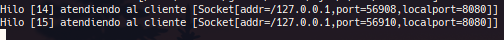
\includegraphics[width=0.8\linewidth]{hilo-por-operacion.png}
    \caption{Consola del servidor, atendiendo varios clientes concurrentemente}
\end{figure}

~\\
\emph{Determine si la implementación del ejercicio 3.- tiene un thread por requerimiento, por conexión, o por recurso} 
~\\

Cuando el servidor acepta una conexión entrante, crea un hilo para atenderla; por lo tanto se podría decir que la implementación del servidor concurrentemente maneja \textbf{un hilo por conexión}. Sin embargo, en cada conexión se realiza \textbf{una única operación} (abrir un archivo, leer un archivo abierto, escribir en un archivo abierto, o cerrar un archivo abierto), así que se podría argumentar que el hilo es \textbf{por requerimiento}. 

~\\
\emph{Comparación en la transferencia de archivos grandes} 
~\\

Comparando ambas implementaciones con un archivo de 3.9GB, los rendimientos cambian considerablemente. Cabe destacar que toda la comunicación que se lleva a cabo con la implementación en C es resuelta por \emph{rpcgen}, por lo tanto se podría suponer que es más performante que la versión de Java. La primer versión comunica el cliente con el servidor mediante UDP, mientras que la segunda versión (Java) trabaja con TCP.

Trabajando con un tamaño de buffer de aproximadamente 8KB, la implementación con RPC transfiere el archivo en \textbf{alrededor de 17 minutos} 

\begin{figure}[h]
    \centering
    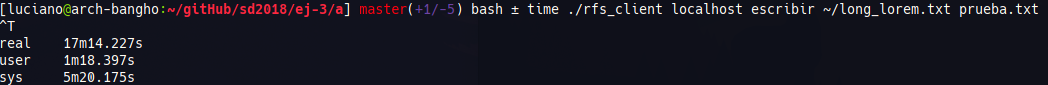
\includegraphics[scale=0.5]{transferencia-rpc.png}
    \caption{3.9GB transferidos en 17 minutos}
\end{figure}

Por otro lado, la implementación en Java demora una cantidad de tiempo cuantiosamente mayor. No estaría demás comentar que esta versión transporta a través de la red varios datos innecesarios (debido a una simplificación en el código). Por ejemplo, cuando se ejecuta una función de lectura, el cliente crea el arreglo de \texttt{byte} y lo envía al servidor; el servidor se encarga de llenar ese arreglo y devolverlo al cliente. 

En un intento de transferir el mismo archivo, en aproximadamente 37 minutos se transfirieron \textbf{400MB de un archivo de 3.9GB}.

\begin{figure}[h]
    \centering
    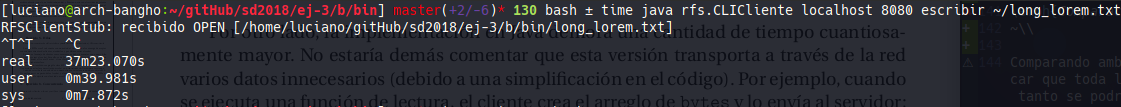
\includegraphics[scale=0.47]{transferencia-java.png}
    \caption{Transferencia cancelada}
\end{figure}
\begin{figure}[h]
    \centering
    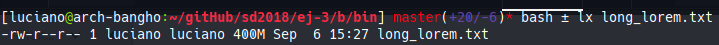
\includegraphics[scale=0.7]{archivo-transferido-java.png}
    \caption{Sólo se transfirieron 400MB en 37 minutos}
\end{figure}

Esta diferencia abismal de velocidades se debe principalmente al \textbf{tamaño del buffer}. Otro experimento realizado fue hacer la misma transferencia (con la versión en Java), pero con un buffer de transferencia de 1MB. Con este cambio, esta versión termina prevalenciendo por sobre la de RPC.

\begin{figure}[H]
    \centering
    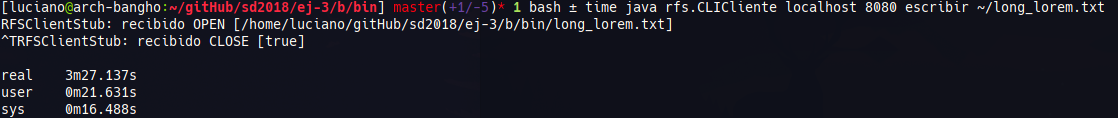
\includegraphics[scale=0.45]{transferencia-java-buffer-grande.png}
    \caption{Archivo transferido en \textbf{3 minutos y medio} }
\end{figure}

Por último, la tercer versión (directorio \emph{comunicación\_performante}), modifica la forma en la que se comunica el cliente con el servidor, únicamente enviando los datos necesarios. Por ejemplo, cuando se desea leer un archivo, el cliente envía el archivo que desea leer (que es el archivo que le devolvió el servidor cuando lo quiso abrir) y la cantidad de bytes; el servidor devuelve un arreglo de \texttt{byte} con los datos pedidos.


\section{\emph{Pool} de hilos}

Implementando el manejo concurrente de clientes con un \emph{pool} de \emph{n} hilos (cantidad fija de hilos previamente creados), se podrá atender hasta \emph{n} de forma concurrente; los \emph{n+1} clientes siguientes serán encolados hasta que se libere uno de los hilos. 

Utilizando esta alternativa, se establece de antemano una cantidad máxima de clientes concurrentes que se podrán manejar. Si se decidiese no hacerlo, una cantidad infinita de clientes podría querer conectarse con el servidor, logrando que se le agote la memoria o que deje de brindar servicio.








%%%%%%%%%%%%%%%%%%%%%%%%%%%%%%%%%%%%%%%%%%%%
% FIN DOCUMENTO, AHORA REFERENCIAS
%%%%%%%%%%%%%%%%%%%%%%%%%%%%%%%%%%%%%%%%%%%%
\clearpage
\printbibliography

\end{document}

